\chapter{Schlussbetrachtung}
\section{Diskussion des Gesamtergebnis}
Eines der Ziele, ein generisches Simulations-Framework für Flugzeuge in C++ zu implementieren wurde dadurch erreicht, dass sämtliche Parameter aus Input-Files eingelesen werden und die Methoden sehr allgemein gehalten wurden. Durch den modularen Aufbau können die einzelnen Module jederzeit um weitere Klassen erweitert werden. Die Simulation selber kann über ein Input-File gesteuert werden, womit unterschiedliche Modelle und Ausbaustufen simuliert werden können, ohne dass der Nutzer den Code selbst verändern muss. In Kapitel \ref{ch:opt} wurde die Performance Optimierung der Simulation erläutert. Das Ziel, die Rechenzeit gegenüber Matlab  zu verbessern und im Nachgang weiter zu optimieren wurde erfüllt, wie in Abbildung \ref{fig:optergeb} zu sehen ist. 
\begin{figure}[h]
	\centering
	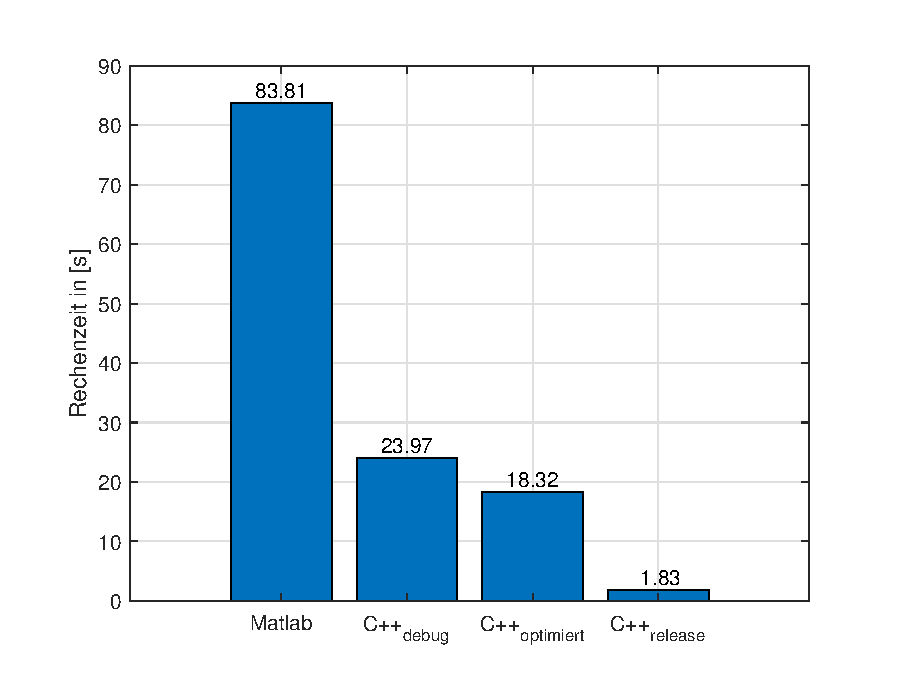
\includegraphics[width=0.7\linewidth]{untitled}
	\caption{Vergleich der Rechenzeiten}
	\label{fig:optergeb}
\end{figure}\noindent\\
Durch die Kompilierung als Release, konnte nochmals ein erheblicher Performancegewinn erzielt werden. Quantitative ergibt sich dadurch eine Rechenzeiteinsparung von 97,2\% gegenüber Matlab.
\section{Erweiterungsmöglichkeiten}
Das Simulationsframework kann aufgrund des modularen Aufbaus jederzeit um weitere Klassen ergänzt werden. Es wurde bereits erwähnt, dass die höchste Ausbaustufe derzeit noch keine Fehlermodelle der Subsysteme besitzt. Diese und auch andere Erweiterungen könnten in Zukunft implementiert werden. Derzeit werden die Unit- und Modultests nur manuell durchgeführt. Eine Automatisierung der Tests wäre denkbar. 
\section{Fazit}
Die in dieser Arbeit gesetzten Ziele wurde mit Erfolg erfüllt. Die Verwendung von Polymorphie wird als sehr effektiv angesehen, um ein Programm modular aufzubauen und um Code zu sparen. Zudem haben sich die in \cite{Kessler.Sommersemester2017} vorgestellten Tools zur effizienten Programmierung bewährt. Die zusätzlich Codedokumentation erwies sich als zusätzliche Last und fordert eine gewisses Maß an Selbstdisziplin. Durch die Durchführung von Unit- und Modultests, konnte die Funktion einiger Methoden nachgewiesen werden. Dennoch ist es sehr schwierig die Tests so zu definieren, um eine große Codeabdeckung zu gewährleisten. Der Leistungsprofiler ist sehr empfehlenswert, um Schwachstellen im Code zu erkennen und nachträglich algorithmisch zu optimieren. Die Möglichkeit der Parallelisierung konnte in dieser Ausarbeitung aufgrund des physikalischen Hintergrunds der Simulation nicht genutzt werden. Zusammenfassend lässt sich sagen, dass dem Nutzer eine funktionsfähige Simulationsumgebung für Flugzeuge zur Verfügung gestellt wird. 


